\section{Recognizing observed actions}
\label{sec:recognition}

The recognition of actions in videos is a fundamental computer vision research theme. Relevant tasks focus on different aspects of the actions observed in full. We start by discussing approaches for optimizing model inputs in \Cref{sec:recognition::inputs}. We then overview popular temporal-based recognition tasks in \Cref{sec:recognition::temporal}. Tasks based on the semantic relationships between language and video are discussed in \Cref{sec:recognition::language}, whereas audio-visual and other multimodal approaches appear in \Cref{sec:recognition::audio}. 

\subsection{Video reduction methods}
\label{sec:recognition::inputs}

% Why sample/reduce compute?

Video inputs typically consist of tens to hundreds of highly visually similar frames. The uniform use of all frames can lead to an unsustainable computational burden. However, humans process stimuli selectively \pcite{eagleman2010does}. 
Several recognition approaches, as shown in \Cref{fig:redundancies_reduction}, aim to reduce compute and improve memory utilization by considering inputs selectively.


% Main challenges in input reduction
\subsubsection{Challenges}
\label{sec:recognition::challenges} 

%Frames in videos introduce redundancies. 
Reducing frame-level redundancies in videos requires a high-level understanding of each temporal segment's relevance. The distinction and selection of relevant segments directly impact information loss. Long and complex scenes present significant challenges to video reduction methods. This \textit{uneven context inclusion} requires more efficient utilization of the model's capacity.

\begin{figure}[t]
     \centering
     \begin{subfigure}[b]{0.49\linewidth}
         \centering
         \includegraphics[width=\linewidth]{figs/redundancies_reduction/redudancies_sample.pdf}
         \caption{\textbf{Frame Sampling}}
         \label{fig:redundancies_reduction::sampling}
     \end{subfigure}
     \hfill
     \begin{subfigure}[b]{0.49\linewidth}
         \centering
         \includegraphics[width=\linewidth]{figs/redundancies_reduction/redudancies_preview.pdf}
         \caption{\textbf{Audio previewing}}
         \label{fig:redundancies_reduction::preview}
     \end{subfigure}
     \\
     \begin{subfigure}[b]{0.49\linewidth}
         \centering
         \includegraphics[width=\linewidth]{figs/redundancies_reduction/redudancies_permute.pdf}
         \caption{\textbf{Video input permuting}}
         \label{fig:redundancies_reduction::permute}
     \end{subfigure}
     \hfill
     \begin{subfigure}[b]{0.49\linewidth}
         \centering
         \includegraphics[width=\linewidth]{figs/redundancies_reduction/redudancies_transfer.pdf}
         \caption{\textbf{Knowledge transfer}}
         \label{fig:redundancies_reduction::transfer}
     \end{subfigure}
        \caption{\textbf{Redundancy reduction methods} include (a) selection of task-specific salient frames, (b) use of supplementary modalities such as audio to preview relevant regions to sample from, (c) input permutations to compress irrelevant frames and segments, and (d) using embeddings from a teacher model as targets.}
        \label{fig:redundancies_reduction}
\end{figure}



\subsubsection{Approaches}
\label{sec:recognition::approaches}

% Frame sampling
Among the most common approaches for reducing redundancies is \emph{frame sampling}. Works on frame sampling rely on policy networks that select frames based on the action's complexity \pcite{ghodrati2021frameexit,yeung2016end}, video context correspondence \pcite{wu2019adaframe}, or changes in the target class' probability \pcite{korbar2019scsampler}. \tcite{wang2021adaptive} used a recurrent network to localize action-relevant regions. Subsequent extensions targeted early stopping \pcite{wang2022adafocus} and related local and global features to determine action-relevant patches \pcite{wang2022adafocusv3}. \tcite{xia2022nsnet} used pseudo labels obtained by computing the embedding distance to class centroids to distinguish individual frames as salient and non-salient. Other approaches have used reward functions based on predictions from the selected frames \pcite{wu2020dynamic}, combined frame-level and video-level predictions \pcite{gowda2021smart}, optimized towards balancing accuracy and number of frames used \pcite{wu2019liteeval}, or removed tokens in transformer architectures \pcite{wu2024haltingvt}. 

% Sampling by using an additional low-cost signal
A related set of approaches has extended unimodal frame sampling with \emph{audio previewing}. \tcite{gao2020listen} used both frame and audio features with a recurrent network to predict the next informative moment in the video. The video resolution used by the model was determined based on discovered informative parts in the audio stream. Similarly, \tcite{nugroho2023audio} used a saliency loss to localize the informative audio segments from which the corresponding video frames can be sampled. 

% Permuting the input (w/o sampling) to improve efficiency
Although coarse frame sampling can be beneficial in short videos, selecting a limited number of frames in longer videos with a broader context can result in information loss. Another line of research thus studies redundancy reduction through \emph{video input permutations}. These works change frame resolutions based on classifier confidence \pcite{meng2020ar} or quantize frames at different precision \pcite{abati2023resq,sun2021dynamic}. \tcite{zhang2022look} used a two-branch approach for lightweight computations over large, less-relevant segments, and assigned more compute for segments with relevant context similar to \pcite{feichtenhofer2019slowfast}.  

% Using teacher model embeddings
Recent efforts have also used \emph{knowledge distillation} to improve the training efficiency of video model pipelines. \tcite{ma2022rethinking} reduced computations by learning to match student network features from videos with reduced resolution to the full-resolution features from a teacher network. \tcite{kim2021efficient} extended this approach by using cross-attention to learn the correspondence between teacher and student features. Distillation approaches have also used non-vision teacher models. \tcite{lei2021less} bound language embeddings to sparsely sampled clips from long videos while \tcite{xia2022temporal} used embeddings from textual event-object relations to discover salient frames. \tcite{tan2023egodistill} proposed a reconstruction approach for interpolating egocentric video features using embeddings from partial frames and the camera motion for the unobserved frames.

\subsubsection{Future outlooks}
\label{sec:recognition::outlooks}

Context-aware models can significantly improve both processing times and performance. Although most video reduction methods are primarily evaluated on classification or detection, more recent action understanding models have been optimized on multi-task and multi-domain objectives. This makes the discovery of relevant frames more difficult. For example, suppressing background frames is sub-optimal for episodic memory in which specific locations or attributes of objects not directly relevant to a current action need to be inferred. We expect that future redundancy reduction methods will focus more on preserving general scene information rather than ensuring that semantics of objects in the scene are not lost. This can be potentially achieved by discovering informative frames for diverse tasks or distilling scene context in low-memory representations, \eg language embeddings.      


\begin{figure*}[t]
    \centering
    \begin{overpic}[width=\linewidth, trim={0 17cm 0 5cm},clip]{figs/localization_detection_counting.pdf}
    \put (15,0) {(a) TAL}
    \put (43,0) {(b) STAD}
    \put (71,0) {(c) VRC}
    
    \end{overpic}
    \caption{\textbf{Visualization of temporal-based tasks}. (a) Temporal Action Localization (TAL) discovers the start and end times of individual actions. In contrast, (b) Spatio-Temporal Action Detection (STAD) is more complex as it requires temporally and spatially localizing actions with bounding boxes for actors and objects over time. Distinctively, (c) Video Repetition Counting (VRC) is not based on action labels and instead requires counting repetitions of actions or motions in an open-set setting. Video source from \tcite{kay2017kinetics}.}
    \label{fig:loc_det_count}
\end{figure*}

\subsection{Temporal-based tasks}
\label{sec:recognition::temporal}

The perception of actions across time is a complex capability of human cognition. Understanding the timing of events is crucial for developing motor memory \pcite{eagleman2010does} for actions such as moving, speaking, and determining the causality of perceived temporal patterns.  
The importance of processing temporal information efficiently by computer vision systems has been shown through both standard performance metrics and semantic benchmarks \pcite{albanie2020end,stergiou2023leaping}. We provide a visualization of temporal-based tasks in \Cref{fig:loc_det_count} with the main challenges and task details discussed below.

% Main challenges in AR
\subsubsection{Challenges}
\label{sec:recognition::temporal:::challenges}

For most tasks, action categories are inferred directly without an explicit notion of their complexity based on \textbf{levels of abstraction}, \eg, atomic movements, composite motions, singular actions, or general activities. Although some datasets include action hierarchies \pcite{shao2020finegym,li2018resound}, these relationships are only used by a handful of existing works \pcite{mettes2020searching}. Different levels of abstraction typically have different temporal ranges, which require different approaches to process visual inputs. Moreover, there can be substantial temporal variations across class instances. This leads to larger temporal distances between discriminative information in videos, requiring proper extraction and modeling of long-range dependencies. We discuss solutions to cope with these variations in this section.

% TAL definition and early works
\subsubsection{Temporal localization} 
\label{sec:recognition::temporal:::localization}

A well-established video task is the discovery and classification of the actions performed alongside their temporal segments. Temporal Action Localization (TAL) aims to infer the action categories alongside the start and end times of the corresponding locations in untrimmed videos. 


Early attempts have used Improved Dense Trajectories \pcite{wang2013action} and Fisher vectors \pcite{oneata2013action} to model the temporal dynamics of local points in scenes. \tcite{shou2016temporal} was one of the first to approach TAL with a joint action proposal and classification objective with a regional CNN. This joint optimization has been adapted with spatial- and temporal-only networks \pcite{lin2018bsn,paul2018w,wang2017untrimmednets}, regional proposal selection \pcite{chao2018rethinking,xu2017r}, and intra-proposal relationships with graph convolutions \pcite{zeng2019graph} in subsequent works. \tcite{shou2017cdc} predicted granularities at a frame level by transposing the temporal resolution of pretrained video encoders. More recent approaches for TAL can be categorized into three broad categories. 

% Single-stage approaches
\noindent
\textbf{One-stage}. Most similar to the aforementioned methods, one-stage approaches localize and classify actions in a single step by using hierarchical embeddings from feature pyramids \pcite{lin2021learning,liu2020progressive,shi2023tridet,zhang2022actionformer} or relating relevant video segments \pcite{shou2018autoloc,yang2020localizing}. Recently, \tcite{yan2023unloc} integrated scene semantic context for TAL with the inclusion of vision-language encoders. The start and end frames of an action can often be ambiguous. A set of approaches have relaxed deterministic start-end times objectives either by weighing the training loss with the importance of each frame \pcite{shao2023action} or by
learning distributions of possible start and end times \pcite{moltisanti2019action}. These approaches aimed to introduce a variance prior to the typical duration of the action. 

% Two-stage approaches
\noindent
\textbf{Two-stage}. Two-stage approaches disentangle the optimization into separate parts. \tcite{zhai2020two} combined proposals from spatial- and temporal-only streams into a fused final prediction. \tcite{chen2022dcan} used long- and short-range temporal information to refine the confidence of the generated action proposals. \tcite{huang2019decoupling} decoupled classification and localization to two objectives during training with two separate models that use cross-modal connections for exchanging information. Some works have focused on maximizing the embedding difference between representations of frames from action segments and non-relevant frames, either with positive and negative instances \pcite{luo2020weakly,zhang2021cola} or by a scoring function \pcite{rizve2023pivotal}. Methods have also improved the features of backbone encoders with TAL-relevant pretext tasks \pcite{zhang2022unsupervised}. Several two-stage methods process videos holistically \pcite{alwassel2021tsp,he2022asm,liu2021weakly,qing2021temporal}. \tcite{alwassel2021tsp} encoded local features over a sliding window using aggregated features from multiple local encoders. The model was optimized with a dual objective for discovering action regions and classifying every segment. Graphs have also been adopted for TAL with \tcite{bai2020boundary} using generated candidate proposals for the graph's start and end edges and their connected nodes. \tcite{zhao2021video} created a graph of hierarchical features over multiple temporal resolutions. More recent approaches \pcite{nag2023difftad} have formulated proposal prediction as a denoising task with noisy action proposals as input to a diffusion model conditioned on the video. Recent approaches have also used pretrained LLMs for TAL with specific Contrastive Language-Image pretraining (CLIP) query embeddings \pcite{ju2022prompting}, video representation masks adapted to the CLIP text encoder space \pcite{nag2022zero}, and CLIP text and visual features that are correlated to foreground masks learned from the video \pcite{phan2024zeetad}.

% Encoder-decoder/DETR
\noindent
\textbf{DEtection TRansformers (DETR)}. A recent set of methods is based on adapting image-based DETR \pcite{carion2020end} to TAL. These approaches rely on transformer encoder-decoders to create regional proposals optimized with bipartite matching. \tcite{tan2021relaxed} adapted DETR to video with a matching scheme of multiple positive action proposals to address sparsity in temporal annotations. Subsequent works have optimized the detection pipeline by either including dense residual connections \pcite{zhao2023re2tal} or caching short-term features \pcite{cheng2022tallformer,hong2022spotting}. 
\tcite{liu2024end} increased the model capacity by training intermediate adapters propagating information to the decoder from intermediate frozen encoder layers. Approaches have also explored training recipes with sparsely updating model layers \pcite{cheng2022stochastic}, vision-language pretraining distillation \pcite{ju2023distilling}, proposal hierarchies \pcite{wu2023newsnet},
and end-to-end TAL encoder-decoder optimization \pcite{liu2022empirical}. Works aiming to reduce training requirements have also been based on language embeddings with tuned visual-language projectors \pcite{liberatori2024test} and by start/end queries \pcite{aklilu2024zero}.



\subsubsection{Spatiotemporal detection} 
\label{sec:recognition::temporal:::detection}

SpatioTemporal Action Detection (STAD) is related to TAL but aims to jointly localize actions temporally and spatially detect action-relevant actors and objects. The main challenge of STAD methods is consistently linking detections and temporal action proposals across frames. Similar to TAL, two general directions can be used to overview relevant literature. 


\noindent
\textbf{Two stages}. Building upon the advancements of image-based object detectors \pcite{girshick2014rich,girshick2015fast}, the majority of STAD approaches first detect objects and then temporally localize actions by tracking object candidates~\pcite{jain2014action,weinzaepfel2015learning}, ROI-pooling RGB and flow features \pcite{peng2016multi}, refining proposals iteratively \pcite{soomro2015action}, aligning source and target domain features~\pcite{agarwal2020unsupervised}, or using the general action level in the video as context \pcite{mettes2016spot}. \tcite{li2018recurrent} built upon prior two-stage detection works and incorporated recurrent proposals to include temporal context. Other approaches that focus on temporal information \tcite{singh2017online} used the arrow of time with different portions of the video detected at each step. Later benchmarks included longer videos to focus on activity-related tasks \pcite{gu2018ava}, enabling the greater exploration of context with feature banks \pcite{feng2021relation,pan2021actor,tang2020asynchronous,wang2018videos,wu2019long,wu2022memvit} and supplementary object information \pcite{arnab2021unified,hou2017tube,zhang2019structured}. Additional information such as keyframe saliency maps~\pcite{li2020actions,ulutan2020actor}, hands and poses~\pcite{faure2023holistic}, actor-object relations~\pcite{sun2018actor}, and SSL~\pcite{wang2023videomae} have also been explored. \tcite{alwassel2018diagnosing} analyzed the benefits of two-stage approaches and showed that they are primarily performant in handling temporal context. However, they also note that a significant limitation of two-stage approaches is that features are computed from backbones trained over auxiliary video tasks, potentially missing specific discriminative information.


\noindent
\textbf{Single-stage}. Drawing inspiration from single-stage object detection methods~\pcite{carion2020end,redmon2016you,liu2016ssd}, single-stage STAD approaches use an end-to-end trained unified framework for joint localization and detection~\pcite{chen2021watch,girdhar2019video,zhu2024dual}. \tcite{ntinou2024multiscale} extended the bipartite matching loss from \tcite{carion2020end} to spatio-temporal tokens. Other approaches used adaptive feature sampling~\pcite{wu2023stmixer}, conditionally modeled visual features based on motion~\pcite{zhao2019dance}, and contrasted different views~\pcite{kumar2022end}. Directly predicting tubelets has also been adopted by recent approaches \pcite{gritsenko2024end,kalogeiton2017action,song2019tacnet,yang2019step,zhao2022tuber}. \tcite{kalogeiton2017action} stacked embeddings from a backbone applied over a sliding window and regressed both classes and tubelets over the entire video. \tcite{zhao2022tuber} used an encoder-decoder to generate tubelet queries and cross-attended them to visual features. \tcite{gritsenko2024end} generated candidate tubelets from condensed query representations cross-attended by features from each frame. Beyond STAD, tubelets have also been used as a self-similarity pretraining objective~\pcite{thoker2023tubelet} to enforce correspondence of videos from different domains but with similar local motions. 

\subsubsection{Repetition counting}
\label{sec:recognition::temporal:::vrc}

Video Repetition Counting (VRC) aims to count the number of action repetitions. In contrast to TAL and STAD, VRC is an open-set task and does not require action categories.





\newcolumntype{g}{>{\columncolor{LightGrey}}l}

\begin{table*}[t]
    \centering
    \caption{\textbf{Self-Supervised Learning (SSL) methods and video task adaptations}. Three learning paradigms are used to group pretext tasks.
    }
    \resizebox{\linewidth}{!}{
    \setlength\tabcolsep{1.0pt}
    \begin{tabular}{c l l c l l }
    \toprule
      Learning & & Task & & Method & Video adaptations~$\textcolor{red}{^1}$  \\
      \midrule
      \multirow{5}{*}{Context-based} & \multirow{5}{*}{       
    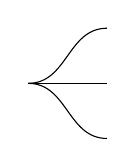
\begin{tikzpicture}
    \draw    (0,.5) .. controls (.5,.5) and (.5,1.2) .. (1,1.2) ;
    \draw    (0,.5) .. controls (.5,.5) and (.5,-.2) .. (1,-.2) ;
    \draw    (0,.5) -- (1,.5) ;
    \end{tikzpicture}
      }&  Arrow of Time & & & \makecell[l]{
      \citet{benaim2020speednet},
      \citet{dwibedi2018temporal},
      \citet{destro2024cyclecl},
      \citet{donahue2024learning}, \\
      \citet{salehi2023time},
      \citet{wei2018learning},
      \citet{wu2021contrastive}
      }  \tstrut \bstrut \\
      & & \multicolumn{1}{g}{Jigsaw} & \multicolumn{1}{g}{} & \multicolumn{1}{g}{} & \multicolumn{1}{g}{\tabularCenterstack{l}{
      \citet{kim2019self},
      \citet{lee2017unsupervised},
      \citet{liu2024solving},
      \citet{misra2016shuffle},
      \citet{wang2022video}, \\
      \citet{xu2019self}
      }} \tstrut \bstrut \\
      & & Colorization & & & \makecell[l]{
      \citet{ali2023task},
      \citet{dhiman2023corf},
      \citet{jabri2020space},
      \citet{liu2024temporally},
      \citet{vondrick2018tracking},\\
      \citet{wu2020memory},
      \citet{zhang2023temporal}
      } \tstrut \bstrut \\
      \multirow{16}{*}{Contrastive} & \multirow{16}{*}{       
    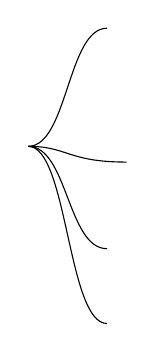
\begin{tikzpicture}
    \draw    (0,0.5) .. controls (.5,0.5) and (.5,2.) .. (1,2.) ;
    \draw    (0,.5) .. controls (.5,0.5) and (.5,.3) .. (1.25,.3) ;
    \draw    (0,.5) .. controls (.5,.5) and (.5,-.8) .. (1,-.8) ;
    \draw    (0,.5) .. controls (.5,.5) and (.5,-1.75) .. (1,-1.75) ;
    \end{tikzpicture}
      }&\multirow{8}{*}{Negative Samples} & \multirow{8}{*}{       
    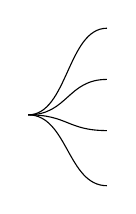
\begin{tikzpicture}
    \draw    (0,-.1) .. controls (.5,-.1) and (.5,1) .. (1,1) ;
    \draw    (0,-.1) .. controls (.5,-.1) and (.5,.35) .. (1,.35) ;
    \draw    (0,-.1) .. controls (.5,-.1) and (.5,-.3) .. (1,-.3) ;
    \draw    (0,-.1) .. controls (.5,-.1) and (.5,-1) .. (1,-1) ;
    \end{tikzpicture}
      } & \multicolumn{1}{g}{MoCo \citep{he2020momentum}} & \multicolumn{1}{g}{\tabularCenterstack{l}{
      \citet{feichtenhofer2021large},
      \citet{han2020memory},
      \citet{kuang2021video}, 
      \citet{liu2021hit},\\
      \citet{ma2021active},
      \citet{pan2021videomoco},
      \citet{qian2021spatiotemporal},
      \citet{xu2021rethinking},
      \citet{yao2021seco} }} \tstrut \bstrut \\
      && && SimCLR \citep{chen2020simple} & \makecell[l]{
      \citet{badamdorj2022contrastive},
      \citet{chen2021rspnet},
      \citet{han2020self},
      \citet{jenni2021time}, \\
      \citet{sun2021composable},
      \citet{wang2020self},
      \citet{yang2020video},
      \citet{zhang2021video}
      } \tstrut \bstrut \\
      && && \multicolumn{1}{g}{CPC \citep{oord2018representation}} & \multicolumn{1}{g}{\tabularCenterstack{l}{
      \citet{akbari2021vatt},
      \citet{bagad2023test}
      \citet{dave2022tclr},
      \citet{li2021motion},
      \citet{miech2020end}, \\
      \citet{park2022probabilistic},
      \citet{parthasarathy2023self},
      \citet{yang2021taco}}} \tstrut \bstrut \\
      && && DIM \citep{hjelm2018learning} & \makecell[l]{
      \citet{bai2022salient},
      \citet{cai2022heterogeneous},
      \citet{feng2023mutual},
      \citet{gordon2020watching}, \\
      \citet{hjelm2020representation},
      \citet{nan2021interventional},
      \citet{sameni2023spatio},
      \citet{sun2019learning}
      } \tstrut \bstrut \\
      && Clustering & \multirow{1}{*}{ 
    \begin{tikzpicture}
    \draw   (0,0.6) -- (1,.6) ;
    \end{tikzpicture}
      } & \multicolumn{1}{g}{SwAV \citep{caron2020unsupervised}} & \multicolumn{1}{g}{
      \tabularCenterstack{l}{
      \citet{coskun2022goca},
      \citet{diba2021vi2clr},
      \citet{long2023cross},
      \citet{toering2022self},\\
      \citet{wei2022inter},
      \citet{yan2020clusterfit}
      }
      } \\
      && \multirow{4}{*}{Self-Distillation} & \multirow{4}{*}{ 
    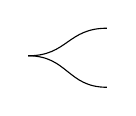
\begin{tikzpicture}
    \draw    (0,.5) .. controls (.5,.5) and (.5,.85) .. (1,.85) ;
    \draw    (0,.5) .. controls (.5,.5) and (.5,.1) .. (1,.1) ;
    \end{tikzpicture}
      }& BYOL \citep{grill2020bootstrap} & \makecell[l]{
      \citet{escontrela2023video},
      \citet{liu2022funnynet},
      \citet{morales2022leveraging},
      \citet{recasens2021broaden},\\
      \citet{ranasinghe2022self},
      \citet{sarkar2023uncovering},
      \citet{xiong2021self},
      \citet{zhang2022contrastive}
      } \\
       && && \multicolumn{1}{g}{DINO \citep{caron2021emerging}} & \multicolumn{1}{g}{\tabularCenterstack{l}{
       \citet{ding2024betrayed},
       \citet{fan2023unsupervised},
       \citet{huang2024vbench},
       \citet{huang2024uvis},\\
       \citet{ponimatkin2023simple},
       \citet{teeti2023temporal},
       \citet{wang2024videocutler}
       }} \\
       && \multirow{2}{*}{Decorrelation} &\multirow{1}{*}{ 
    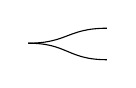
\begin{tikzpicture}
    \draw    (0,.66) .. controls (.5,.66) and (.5,.85) .. (1,.85) ;
    \draw    (0,.66) .. controls (.5,.66) and (.5,.45) .. (1,.45) ;
    \end{tikzpicture}
      } & Barlow Twins \citep{zbontar2021barlow} & \multirow{1}{*}{
      \citet{da2022unsupervised},
      \citet{peh2024learning},
      \citet{zhang2022contrastive},
      \citet{zhou2023self}
      } \\
       && && \multicolumn{1}{g}{VICReg \citep{bardes2021vicreg}} & \multicolumn{1}{g}{
       \multirow{1}{*}{
       \citet{bardes2023mc},
       \citet{sun2023unified},
       \citet{yang2023contrastive},
       \citet{yu2024evolve}
       }
       } \\
       \multirow{7}{*}{Masking} &
       \multirow{7}{*}{       
    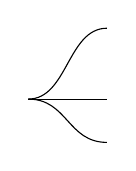
\begin{tikzpicture}
    \draw    (0,1.8) .. controls (.5,1.8) and (.5,2.7) .. (1,2.7) ;
    \draw    (0,1.8) .. controls (.5,1.8) and (.5,1.8) .. (1,1.8) ;
    \draw    (0,1.8) .. controls (.5,1.8) and (.5,1.25) .. (1,1.25) ;
    \end{tikzpicture}}
    & \multirow{2}{*}{low-level targets} & \multirow{1}{*}{ 
    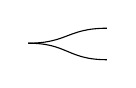
\begin{tikzpicture}
    \draw    (0,.66) .. controls (.5,.66) and (.5,.85) .. (1,.85) ;
    \draw    (0,.66) .. controls (.5,.66) and (.5,.45) .. (1,.45) ;
    \end{tikzpicture}
      }& ViT \citep{dosovitskiy2020image} & \makecell[l]{
      \citet{girdhar2023imagebind},
      \citet{lin2022frozen},
      \citet{piergiovanni2023rethinking}
      } \\
       && && \multicolumn{1}{g}{MAE \citep{he2022masked}} & \multicolumn{1}{g}{\tabularCenterstack{l}{
       \citet{feichtenhofer2022masked}, \citet{girdhar2023omnimae}, \citet{huang2023mgmae}, \citet{huang2023mavil}, \\ \citet{ryali2023hiera},  \citet{tong2022videomae}, \citet{wang2023videomae}, \citet{wu2023dropmae}}} \\
       && high-level targets & \multirow{1}{*}{ 
    \begin{tikzpicture}
    \draw    (0,.85) .. controls (.5,.85) and (.5,.85) .. (1,.85) ;
    \end{tikzpicture}
      }& BEiT \citep{bao2021beit} & \makecell[l]{
      \citet{cheng2023vindlu},
      \citet{fu2021violet},
      \citet{li2023svitt},
      \citet{tan2021vimpac},
      \citet{wang2022bevt}
      } \\
       && \multirow{2}{*}{Teacher-based} &\multirow{1}{*}{ 
    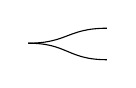
\begin{tikzpicture}
    \draw    (0,.66) .. controls (.5,.66) and (.5,.85) .. (1,.85) ;
    \draw    (0,.66) .. controls (.5,.66) and (.5,.45) .. (1,.45) ;
    \end{tikzpicture}
      }& \multicolumn{1}{g}{data2vec \citep{baevski2022data2vec}} & \multicolumn{1}{g}{
      \tabularCenterstack{l}{
      \citet{li2023unmasked},
      \citet{lian2023av}
      }
      } \\
       && && MaskFeat \citep{wei2022masked} & 
       \makecell[l]{
       \citet{feichtenhofer2022masked},
       \citet{mizrahi20234m},
       \citet{lin2023smaug},
       \citet{pei2024videomac} \\
       \citet{stergiou2024holistic}, 
       \citet{wang2023masked},
       \citet{woo2023towards},
       \citet{zhao2024asymmetric}
       }  \\
      \end{tabular}
    }
    \label{tab:SSL_tasks}
    \vspace{-1em}
\end{table*}

Early works on signal periodicity \pcite{thangali2005periodic} have decomposed signal repetition with a Fourier analysis \pcite{branzan2008generic,briassouli2007extraction,ousman2008segmentation,ross2000robust,pogalin2008visual}. Signal-based works have also used the direction of motion flow over time \pcite{runia2018real} to count repetitions. Another set of methods approached VRC as a classification task over a finite set of maximum repetitions. \tcite{lu2004repetitive} used dynamic parameters based on the Frobenius norm to classify changes corresponding to action end times.
\tcite{zhang2021repetitive} fused audio and video representations while \tcite{zhang2020context} used multiple cycles to refine the repetition count prediction. \tcite{li2024efficient} extracted action query features and classified the queries by their repetitions. In contrast to defining repetition counts as classes, \tcite{dwibedi2020counting} adopted a temporal self-similarity matrix \pcite{benabdelkader2004gait,junejo2010view,korner2013temporal} to discover repetition periodicity. Subsequent methods have investigated embedding similarity matrices at multiple scales \pcite{bacharidis2023repetition,hu2022transrac}, triplet contrastive losses \pcite{destro2024cyclecl}, and graph representations \pcite{panagiotakis2018unsupervised}. Because embeddings of adjacent frames are highly similar, several recent methods have aimed to limit the discovery of correspondences in repetitions to poses \pcite{ferreira2021deep,yao2023poserac}, specific frames \pcite{li2024repetitive,zhao2024skim}, visual exemplars \pcite{sinha2024every}, or language descriptions \pcite{dwibedi2024ovr}. VRC remains a challenging task given the open-set nature and the lack of robust baselines in recent large-scale datasets \pcite{dwibedi2024ovr}.

\subsubsection{Future outlooks}
\label{sec:recognition::temporal:::outlooks}

Despite the great progress, using unified systems to generalize across tasks remains challenging. For example, STAD methods \pcite{dai2021pdan,tirupattur2021modeling} benchmarked on TAL perform lower than TAL-based models, as their joint objective of localizing both \emph{when} and \emph{where} actions are performed is significantly more challenging to optimize. Similarly, despite the task similarities between TAL and VRC, standard TAL methods do not generalize to VRC as action interruptions and out-of-distribution categories cannot be effectively segmented \pcite{hu2022transrac,sinha2024every}. The recent introduction of unified VLMs for multiple video tasks, e.g., \pcite{wang2024internvideo2} and their use as a feature extractor in subsequent works \pcite{chen2024video}, has shown a promising direction through the use of SSL. Training recipes typically include multiple stages of contrastive and masking pretext self-supervision objectives to allow the generalization of the model to multiple tasks. Training on SSL pretext tasks is a prominent scheme for many video-based models, as shown in \Cref{tab:SSL_tasks}. Context-based approaches rely on inherited spatiotemporal structural relationships in videos. Contrastive objectives are based on instance discrimination tasks, while masking tasks learn representation structures through completion. A possible direction of future research can be the unification of downstream objectives through relevant context, contrastive, and masking pretext tasks based on \emph{the arrow of time}, relationships between task-specific embeddings, or clustering embeddings of semantically similar tasks.     




\subsection{Language semantics in videos}
\label{sec:recognition::language}


LLMs have achieved great success in Natural Language Processing (NLP) and have consequently been adapted for action understanding tasks. The relationships between learned context-rich semantic space and visual world attributes are useful for tasks such as caption generation~\pcite{seo2022end,sun2019videobert,wang2024omnivid}, inferring scene information~\pcite{anderson2018vision,cheng2024egothink}, understanding the general context in highlight detection~\pcite{lei2021detecting}, and instructional video learning~\pcite{miech2020end}. Beyond their direct applicability to language-based tasks, they can incorporate vision encoders~\pcite{ashutosh2023hiervl,fu2021violet,kahatapitiya2024victr,song2024moviechat,xu2021videoclip,zellers2021merlot} learning general and semantically-rich representations that can then be used as feature extractors in downstream tasks. However, notable challenges persist despite the popularity of vision-language semantic similarity pretraining for distilling context into video models. 

\subsubsection{Challenges}
\label{sec:recognition::language:::challenges}

Visual and language information can provide partly complementary perspectives of a video. However, as information from each modality is often heterogeneous, specific representations may not be directly matched through cross-modal correspondence, \eg, due to occluded objects or fine-grained visual details about the performance of the action. Such discrepancies can arise based on domain knowledge specificity or distribution patterns of the available data~\pcite{liang2024foundations}. \textbf{Modality gap}~\pcite{liang2022mind}, shown in \Cref{fig:mod_gap}, is a phenomenon that arises in VLM training in which embeddings of each modality are represented in distinct low-variance regions in the embedding space. In VLMs trained with cross-modal information maximization~\pcite{bain2021frozen,lei2021less,li2020hero,li2022align,zhu2020actbert} this effect becomes stronger with the enforcement of strong coordinate restrictions based on positive and negative cross-modal pairs. This is also relevant to difficulties in the \textbf{cross-modal context alignment} over local elements for tasks with available ground-truth pairs and global representations for tasks without vision-language pairs. In both cases, aligning language and vision context information at either the word/object level or over groups of instances in the embedding space provides a significant challenge in optimization. For generative tasks, this can also lead to difficulties in \textbf{modality-specific generation}. Generating semantic-rich data based on relationships from auxiliary modalities with ambiguous correspondence can impact conditional, stochastic, or auto-regressive generation.

\begin{figure}[t]
    \centering
    \includegraphics[width=\linewidth]{figs/mind_the_gap.pdf}
    \caption{\textbf{VLM modality gap}. Given video encoder $\mathcal{E}_V$ and text encoder $\mathcal{E}_L$, video and text are embedded to $\mathbf{z}_v^{+}$ and $\mathbf{z}_l^{+}$ in a joint embedding space $\mathbb{R}^{\Omega}$. VLM objectives align both $\mathbf{z}_v^{+}$ and $\mathbf{z}_l^{+}$. Contrastive approaches~\pcite{chen2020simple,oord2018representation,xu2021videoclip} additionally maximize the distance between negative vision-language pairs: ($\mathbf{z}_v^{+}$, $\mathbf{z}_l^{-}$) and ($\mathbf{z}_v^{-}$, $\mathbf{z}_l^{+}$). Despite high-level semantic similarity, relevant modality-specific information that is not transferable across modalities can lead to a \emph{modality gap} over embeddings. Videos sourced from \tcite{lei2018tvqa}.}
    \label{fig:mod_gap}
    \vspace{-1em}
\end{figure}


\begin{figure*}
    \centering
    \begin{overpic}[width=\linewidth,keepaspectratio]{figs/retreival_tasks.pdf}
        %\put(2,-1){(a) \textbf{Instance-based}}
        %\put(58,-1){(b) \textbf{Semantics-based}}
        %\put(84,-1){(c) \textbf{TSG}}
    \end{overpic}
    \caption{\textbf{Video retrieval tasks}. (a) Instance-based retrieval returns only a \emph{single video} corresponding to a search query.(b) Semantics-based retrieval returns \emph{a ranking score} corresponding to each video's relevance to the search query. (c) Temporal Sentence Grounding (TSG) receives \emph{video segments from queries} and returns the start and end time per segment. Videos sourced from \tcite{xu2016msr}.}
    \label{fig:retreival_tasks}
\end{figure*}


\subsubsection{Vision-language retrieval} 
\label{sec:recognition::language:::vr}

Video retrieval sources relevant videos from a dataset based on an input query in natural language. As shown in \Cref{fig:retreival_tasks}, research works can be categorized into instance- and semantic-based.


Image methods have explored cross-view ranking~\pcite{wang2016learning}, language to visual attention~\pcite{torabi2016learning}, or visual features as embedding targets for language encodings~\pcite{dong2018predicting}. Early adaptation of visual-language approaches to videos have used image-text-video triplets \pcite{otani2016learning}, and related parts of speech to objects and actions \pcite{gabeur2020multi,xu2015jointly}. 

\noindent
\textbf{Instance-based} approaches use a binary score function to rank correspondences. This formulation assumes only a single relevant caption/video for each video/caption.  Refinements to this objective have been made through visual-language binding with the inclusion of parts-of-speech in target captions \pcite{wray2019fine} and dual object-text and action-text models \pcite{liu2019use,mithun2018learning}. A number of methods have studied vision-language pretraining approaches \pcite{ge2022bridging,lin2022egocentric,xue2022advancing}. \tcite{ge2022bridging} related verbs and nouns to questions and video segments. \tcite{xue2022advancing} studied the correspondences between keyframes and all video frames, subsequently contrasting the keyframe-fused video features to language embeddings.


\noindent
\textbf{Semantics-based}. A more challenging task is to retrieve images based on shared semantics to query images~\pcite{gordo2017beyond}. Semantic-based approaches primarily use triplet losses that contrastively regress between text queries and corresponding positive and negative visual inputs. These methods are based on the similarity between every (video, and caption)
pair. Video retrieval works have studied this through either a contrastive objective based on a support set of videos with similar action categories \pcite{patrick2020support} or a semantic
similarity scoring function for videos from the same category \pcite{wray2021semantic}. Recently, \tcite{kim2024you} have utilized prior knowledge in retrieving text features based on embedding correspondences to similar visual features. \tcite{chun2021probabilistic} proposed probabilistic representations of visual features to accommodate multi-query relevance. Similarly, \tcite{li2023progressive} created an object-phrase and event-phrase prototype-matching framework to enforce relations between high-level concepts across modalities. \tcite{hao2024uncertainty} employed an uncertainty estimate based on the Wasserstein distance between source and target domains of text-vision pairs.


\noindent
\textbf{Temporal sentence grounding (TSG)}. TSG \pcite{regneri2013grounding} localizes moments in videos based on provided natural language queries. Compared to retrieving entire videos, TSG only retrieves relevant segments from a video based on queries. The task closely relates to TAL as also shown by the overlapping works \pcite{gao2017tall} jointly exploring the two tasks. However, in contrast to TAL, TSG requires both natural language reasoning between query and answer, and language-vision reasoning with query-video and answer-video relevance. Following \tcite{gao2017tall}, a broad formulation of TSG includes a visual-language semantic alignment between videos and sentences with a regression loss used for temporal sentence localization.



Early approaches have explored region proposals \pcite{chen2018temporally,qu2020fine,liu2018cross}, ranking \pcite{escorcia2019temporal}, distance-based joint vision-language embeddings \pcite{anne2017localizing,rohrbach2016grounding}, and cross-modal graph representations \pcite{liu2022memory,zhang2019man}. As
the association of visual and text features can be performed at multiple levels of abstraction, subsequent methods have learned correspondences over multiple proposals \pcite{xu2019multilevel}, local and global information \pcite{jiang2019cross,mun2020local}, and word/sentence-level cues \pcite{hao2022query}. \tcite{zhang2021natural} used language-guided highlighting by cross-attending text features to multi-resolution video features. Another important aspect of discovering associations between the two modalities is their conditionality, as visual aspects should depend on the descriptions. Approaches have explored step-wise fusion of language key and value tokens 
\pcite{cao2021pursuit}, localizing relevant video features based on text embeddings \pcite{yang2022tubedetr}, matching video segments and text features contrastively \pcite{flanagan2023learning}, and enforcing similarity between sequential tokens \pcite{qian2024momentor}. \tcite{ge2019mac} used both instance-based vision-language embeddings and general category representations to calculate an actionness score and location offset. Other approaches have fused context from global and local temporal resolutions \pcite{liu2021context}, grounded cues from anchor frames and boundary proposals \pcite{wang2020temporally}, related unimodal and cross-modal representations \pcite{nan2021interventional}, and adopted instance-relevant positional information \pcite{gu2024context}. \tcite{goletto2024amego} explored TSG for language hand-object interaction queries.


\begin{table}[t]
    \centering
    \caption{\textbf{Video captioning papers grouped by target task and overall approach}. Tasks are grouped by the generation of single or dense captions and the specialization to coherency with visual storytelling. Approach denotes architectural and model choices.}
    \resizebox{\linewidth}{!}{
    \setlength\tabcolsep{1.0pt}
    \begin{tabular}{c c l}
    \toprule
      Task & Approach & Works \\
      \midrule
      \multirow{4}{*}{\makecell[c]{Single video \\ captioning}} & \cellcolor{LightGrey}{CNN+LSTM} & \multicolumn{1}{g}{\tabularCenterstack{l}{
      \citet{aafaq2019spatio},
      \citet{chen2017generating},\\
      \citet{gan2017semantic},
      \citet{pan2017video},\\
      \citet{wang2018reconstruction},
      \citet{zheng2020syntax}
      }}\\
      & Trnsf-based & \makecell[l]{
      \citet{lin2022swinbert},
      \citet{shen2023accurate},\\
      \citet{yan2023prompt}
      } \\
      &\cellcolor{LightGrey}{VLM} & \cellcolor{LightGrey}{ \citet{chen2024panda}, \citet{seo2022end}}  \\
      \midrule
      \multirow{3}{*}{\makecell[c]{Dense video\\ captioning}} & \makecell[c]{Region \\ proposals} & \makecell[l]{
      \citet{deng2021sketch},
      \citet{iashin2020better},\\
      \citet{iashin2020multi}
      \citet{krishna2017dense},\\
      \citet{li2018jointly},
      \citet{mun2019streamlined},\\
      \citet{shi2019dense},
      \citet{wang2018bidirectional},\\
      \citet{zhou2018end}
      } \\
      & \cellcolor{LightGrey}{MIL} & \multicolumn{1}{g}{\tabularCenterstack{l}{
      \citet{chen2021towards},
      \citet{shen2017weakly}
      }} \\
      \midrule
      \makecell[c]{Visual\\ storytelling} & VLM & \makecell[l]{ 
      \citet{li2019video},
      \citet{yu2021transitional},\\
      \citet{xiao2022hierarchical} ,
      \citet{han2023autoad},\\
      \citep{han2023autoadii},
      \citep{han2024autoadiii}
      }
      \end{tabular}
    }
    \label{tab:captioning_methods}
    \vspace{-1em}
\end{table}




\subsubsection{Video Captioning} 
\label{sec:recognition::language:::vc}

A long-standing challenge in computer vision is the generation of high-level descriptions in language. In contrast to retrieval tasks that depend on a fixed vocabulary, captioning is a generative task. Starting from matching a small corpus of words to objects in images \pcite{barnard2001learning,barnard2003matching}, current works in the image domain are capable of generating diverse and detailed image descriptions \pcite{mokady2021clipcap,alayrac2022flamingo}. Video captioning includes further challenges as the appearance of objects and the context of scenes change throughout the video. Given the temporal extent of videos, captioning tasks can be divided into two categories (\Cref{tab:captioning_methods}).

\noindent
\textbf{Single video captioning}. A large number of works have studied the direct extension of image captioning to video with single captions.  
Given a video clip and a corresponding caption, a general formulation of a single video captioning objective would be the minimization of the log-likelihood of the caption conditioned on the video.


Initial efforts \pcite{guadarrama2013youtube2text} used semantic hierarchies with word selection through decision tree nodes. Following methods \pcite{aafaq2019spatio,chen2017generating,gan2017semantic,pan2017video,wang2018reconstruction} used encoder-decoder architectures that combined CNNs' visual feature extractors and recurrent architectures (RNNs or LSTMs) to generate textual descriptions. To focus on object semantics, \tcite{aafaq2019spatio,zheng2020syntax} included object detector embeddings. The improved context size of transformers has enabled more recent approaches to explore spatio-temporal dynamics in videos and cross-modal relationships. Transformer approaches have included language supervision over hierarchies \pcite{ye2022hierarchical} and token masking \pcite{lin2022swinbert,shen2023accurate,yan2023prompt}. \tcite{seo2022end} used a VLM with the video encoder and language decoder trained jointly on a reconstruction loss. Recently, \tcite{chen2024panda} explored knowledge distillation from multiple VLM models to generate captions. \tcite{majumder2024viewpoint} jointly learned a viewpoint ranking model for video captioning in multi-view settings.

\begin{figure}[t!]
    \centering
    \includegraphics[width=\linewidth]{figs/CRITIC2.pdf}
    \caption{\textbf{CRITIC metric for visual storytelling}. Identities are obtained from character lists and descriptions fed to a co-referencing model. CRITIC \pcite{han2024autoadiii} is calculated as the IoU between predicted and reference identities.}
    \label{fig:CRITIC}
\end{figure}

\noindent
\textbf{Dense video captioning}. Dense video captioning approaches generate multiple captions and temporally ground them to corresponding video segments. This is a significantly more challenging task as distinct video segments need to be localized to generate corresponding captions. Early works on event localization \pcite{krishna2017dense,li2018jointly,shi2019dense,wang2018bidirectional,zhou2018end} were based on proposal modules from extracted video features. To learn vision-language correspondence explicitly for regions of interest, \tcite{zhou2018end} used proposals as masks for visual and language embeddings. Other approaches improved proposal generation by using their sequential occurrence as a prior \pcite{mun2019streamlined}, deployed feature clipping based on proposals \pcite{iashin2020better,iashin2020multi}, refined general captions for each proposal \pcite{deng2021sketch}, and used unique CLIP properties to generate distinct captions \pcite{perrett2024s}. Overall, proposal-based methods are optimized on a loss that relates the proposal interval to the ground truth segment and a captioning loss. As ground truth proposals require exhaustive annotation efforts, more recent works have focused on proposal-free approaches. \tcite{shen2017weakly} used Multi-Instance Learning (MIL) in which word instances are assigned to bags. They used a binary objective to separate positive bags in which at least one instance corresponds to a target word and negative bags in which no instance contains the target word. MIL has been a building block in subsequent weakly-supervised approaches \pcite{chen2021towards}. Further works \pcite{yang2023vid2seq,ren2024timechat} have also used sequence-to-sequence modeling with learnable time tokens for visual-language relations. \tcite{mavroudi2023learning} combined instruction learning to model the sequentially of video captioning. \tcite{islam2024video} used a two-stage autoregressive approach that first generates dense captions for short clips and then cross-attends them to visual features over longer segments to generate longer captions. \tcite{zhou2024streaming} aimed at efficiency improvements by compressing frame-instance visual features to clusters.


\noindent
\textbf{Visual storytelling}. A recently introduced challenging task that is gaining interest is the generation of coherent sentences for sequential videos \pcite{li2019video}. To bridge cross-modal semantics, \tcite{yu2021transitional} used a coherence loss for past, present, and future frames and contrastively pulled visual and language embeddings closer. A similar contrastive objective was used by \pcite{xiao2022hierarchical} alongside masking part of the visual input. \tcite{han2023autoad} trained a mapping module to project joint CLIP visual features, audio descriptions, and subtitles to an LLM input space to generate captions. Following efforts proposed additional refinements in the pipeline by injecting visual and caption embeddings over multiple LLM layers \pcite{han2023autoadii}, using exemplars \pcite{han2024autoadiii}, and using character-based prompting \pcite{xie2024autoad}. The CRITIC metric, shown in \Cref{fig:CRITIC}, was recently introduced by \tcite{han2024autoadiii} to measure the conceptual alignment of the generated sentences.


\subsubsection{Video Question Answering (VideoQA)}
\label{sec:recognition::language:::vqa}

A widely-used benchmark for VLM models is the utilization of visual context to answer natural language questions \pcite{antol2015vqa,goyal2017making}. In contrast to video captioning, it requires understanding parts of objects and the temporal extent of relevant answers. Depending on the task setting, answers can be obtained from multi-choice QA or as a global answer in open-end QA. 

In a multi-choice QA setting, given a video and a question, the goal is to learn a mapping that returns an answer from a set of possible answers. In open-end QA settings, the answer is instead generated from a model conditioned on the video and question. VQA methods can be divided into two broad groups (\Cref{fig:videoqa}).

\begin{figure}[t!]
    \centering
    \begin{subfigure}[t]{0.5\linewidth}
        \centering
        \includegraphics[width=\textwidth]{figs/graph_vqa.pdf}
        \caption{Graph-based}
    \end{subfigure}%
    ~ 
    \begin{subfigure}[t]{0.5\linewidth}
        \centering
        \includegraphics[width=\textwidth]{figs/vlm_vqa.pdf}
        \caption{Memory-based}
    \end{subfigure}
    \caption{\textbf{VideoQA approaches}. The graph-based approach in (a) is based on the method from \tcite{park2021bridge}. The memory-based approach with a two-stage VLM in (b) is based on \tcite{yu2023self}. Videos sourced from \tcite{xiao2021next}.}
    \label{fig:videoqa}
\end{figure}



\noindent
\textbf{Scene-graphs}. Early VideoQA approaches were based on either graph representations \pcite{jiang2020reasoning,tu2014joint} or on each modality's heterogeneity. \tcite{huang2020location} used object and location-based graph embeddings to relate visual and text features with a cross-modal similarity matrix. Graph representations have also been created from hierarchies of objects and their interactions~\pcite{dang2021hierarchical} as well as over multiple frames~\pcite{liu2021hair}. Alternative approaches defined scales from multiple graph convolution resolutions to relate cross-scale interactions \pcite{guo2021multi} or from subgraphs to capture static and dynamic scene objects  \pcite{cherian20222}. \tcite{park2021bridge} created appearance, motion, and question graphs, learning conditionality by propagating nodes across graphs. Graph representations have also been learned contrastively \pcite{xiao2023contrastive} from positive and negative pairs of video snippets and answers.


\noindent
\textbf{Multimodal memory}. Another set of methods aims to memorize relations between visual and text features across time. Initial efforts integrated additional memory modules in LSTMs \pcite{jang2017tgif,xu2017video,zeng2017leveraging}. Attention-based approaches \pcite{ye2017video} combined modality-specific memory modules~\pcite{fan2019heterogeneous} and memory-sharing modules to cross-attend motion and appearance \pcite{gao2018motion,li2019beyond}. Several works \pcite{gao2023mist,li2023discovering,yang2022zero,xue2023egocentric} have used a single model with concatenated language and vision tokens to predict answers to queries. Recent approaches have adapted large VLMs for VideoQA. \tcite{yu2023self} used a two-stage dual-VLM to first localize video segments based on the video and question and then used only the selected frames and question to generate the answer. Similarly, \tcite{min2024morevqa} used a list of generated VLM captions describing scenes in videos as input to an LLM. The question was then passed as a prompt to discover the most relevant answer. However, recent efforts \pcite{xiao2024can} have also revealed that VLM-based approaches may produce answers based on spurious language correlations and not the visual context.



\subsubsection{Future outlooks}
\label{sec:recognition::language:::outlooks}

Advancements in VLMs have enabled the recognition of actions based on their correspondence to a large lexical corpus. Building upon this correspondence, retrieval, captioning, and question-answering models have moved beyond single-instance structural representations and toward the discovery of abstract cross-modal semantics. The increased model capacity provides opportunities for future lines of research.

Most VLMs strongly rely on linguistic associations that may not be relevant in vision instances \pcite{rahmanzadehgervi2024vision}. A possible alternative is to develop unified multimodal models that tokenize and encode video frames and images in the same manner with positional embeddings also encoding temporal relationships. Initial efforts by \tcite{jang2023unifying} and \tcite{jin2024integration} have been promising. Another direction includes a better exploration of the objectives used. The majority of works train models on objectives \pcite{chen2020simple,he2020momentum,oord2018representation} or using downstream task adapters \pcite{hu2021lora} which can enforce properties such as feature suppression \pcite{chen2021intriguing} and pretext granularity \pcite{cole2022does} despite aiming to maximize correspondence. Crafting better alignment objectives for cross-model representations and semantic relevance can benefit future VLM approaches.  


\subsection{Multimodal recognition} 
\label{sec:recognition::audio}

The recognition of actions or activities has been predominantly studied in the vision domain. In contrast, the auditory recognition of actions from sounds emitted by objects or actors and their interactions is more sparsely researched. This task presents distinct challenges as the sounds emitted by different objects or actions can be similar. 

Time-frequency spectrograms have been a popular format for representing audio events in videos. Initial audio-based models have been built following image-based object recognition \pcite{gong2021psla} or video classification \pcite{kazakos2021slow} CNNs. Attention-based audio methods have used convolutional features \pcite{gulati2020conformer,kong2020panns} or image-pretrained encoders \pcite{koutini2021efficient} to attend over spectrogram patches. Approaches have also explored patch masking \pcite{baade2022mae,huang2022masked}, focused on salient sounds \pcite{stergiou2023play}, and adapted \pcite{liu2022learning_the} or compressed \pcite{feng2024coarse} spectrogram resolutions. More recently, the use of audio has gained attention in multimodal systems as it can provide supplementary information to both visual features and language context. 


\subsubsection{Challenges}
\label{sec:recognition::audio:::challenges}

The use of multiple modalities introduces several challenges. \textbf{Learning cross-modal dynamics} is a fundamental challenge of multimodal models as it aims to preserve heterogeneous properties of modalities while maintaining interconnectivity between modalities \pcite{liang2022foundations}. Fused embedding spaces \pcite{girdhar2023imagebind,girdhar2022omnivore,piergiovanni2023rethinking,zhu2024languagebind} effectively reduce modality-specific information and instead rely on learning a high level of abstraction, with lower heterogeneity and higher interconnectivity. In contrast, modality-specific embedding spaces \pcite{gong2022uavm,gong2023contrastive,chen2024soundingactions,recasens2021broaden} are learned through cross-modal associations and rely on effectively transferring distribution across modalities, causing higher heterogeneity and lower interconnectivity. These paradigms are affected by \textbf{domain-specific noise topologies}. Based on a given task or data distribution, the discriminability of each modality differs. Noise naturally occurs based on environment settings, \eg visual features are more relevant in daylight than in night videos. It can also be observed with instance-based occlusions or sensory imperfections. Such topologies are important when developing reasoning structures over modalities \pcite{gat2021perceptual}. \textbf{Input representation reasoning} can be defined as combining knowledge from the data and the structure of the objective. Compositional relationships between modalities can be established through concept hierarchies, temporal correspondence, or interactive states. Commonly, such structures are not available beforehand and are instead learned in an unsupervised manner.

\begin{figure*}
    \centering
    \begin{overpic}[width=\linewidth,keepaspectratio]{figs/3d_tasks.pdf}
        \put(2,-2){(a) \textbf{3D pose and shape regression}}
        \put(50,-2){(b) \textbf{HOI}}
        \put(75,-2){(c) \textbf{Dynamic scene rendering}}
    \end{overpic}
    \vspace{0.05em}
    \caption{\textbf{4D video understanding tasks}. (a) 3D human pose and shape regression takes as input monocular videos and produces expressive 3D representations. (b) Human/hand-object interactions predict aspects of human-object interactions, such as the contact area or the grasp. (c) Dynamic scene rendering estimates the per-timestep geometry of scenes from sets of images. Figures sourced from \citet{dwivedi2024tokenhmr,fan2024hold,zhang2025monst3r}.}
    \label{fig:4d_tasks}
\end{figure*}

\subsubsection{Audio-visual models} 
\label{sec:recognition::audio:::avmodels}

As video and audio signals differ significantly, works have used two-step models to infer predictions. Two-step approaches extract video and audio embeddings first and then fuse either modality-specific predictions \pcite{fayek2020large}, embeddings from multiple modalities \pcite{xiao2020audiovisual}, or they jointly attend vision and audio features for the final prediction \pcite{gong2022uavm}. More recently, architectures have tokenized and attended audio and vision jointly with multimodal learnable tokens \pcite{nagrani2021attention}, cross-modal attention \pcite{jaegle2021perceiver}, and modality gating \pcite{xue2023dynamic}. To account for models trained on unimodal tasks, \tcite{lin2023vision} proposed cross-modal adapters to combine unimodal embeddings in multimodal tasks. Exploring the relevant audio and visual features with self-supervision has also been a learning paradigm of significant interest. Common embedding spaces can be useful for discovering correspondences in both unimodal and cross-modal retrieval \pcite{arandjelovic2018objects,wu2021exploring}, multimodal clustering \pcite{hu2019deep}, and sound source separation \pcite{hu2022mix,mo2023unified,zhao2018sound}. Token reconstruction through masking has also been used as a self-supervised pretraining task with a variety of training schemes, including concatenating masked tokens \pcite{gong2023contrastive}, multi-view masking per modality \pcite{huang2023mavil}, fusing a mixture of per-modality masked tokens \pcite{guo2024crossmae}, combining modality-specific masked and unmasked embeddings \pcite{georgescu2023audiovisual}, and using multiple masking ratios with siamese networks \pcite{lin2024siamese}. 

Variations in the relevance of visual or auditory signals depend on instances. A promising direction for integrating this into optimization is gradient blending \pcite{wang2020makes} which recalibrates per-modality losses. Other works explored multi-audio to single-visual scene correspondence with contrastive learning. This was done by utilizing joint semantic similarity in both modalities \pcite{morgado2021audio}, using active sampling to diversify negative sample selection
\pcite{ma2021active}, and by counterfactual audio and video pairs to enforce a relationship between multi-audio to single visual scenes \pcite{singh2024looking}. Enforced audio and vision steams similarities can also be used to train models on incremental tasks \pcite{pian2023audio}.



\subsubsection{Gaze and vision models} 
\label{sec:recognition::audio:::gazemodels}

% gaze as saliency cue
Gaze can be used as a saliency cue to direct attention or processing priority towards target focal areas \pcite{itti2002model}. Several egocentric activity datasets \pcite{huang2024egoexolearn,li2018eye,pan2023aria} record gaze as an additional modality. Based on gaze inputs, gaze fixations have been used to recognize objects being manipulated \pcite{land2001ways}, and discover ways of interacting with them \pcite{damen2024youdo}. Observing gaze patterns, including fixations and saccades, in conjunction with scene appearance has also been used to predict future gaze behavior \pcite{huang2018predicting}.

% action prediction from gaze
Because gaze and action are tightly coupled \pcite{vickersadvances}, subsequent research has focused on action recognition with the additional availability of gaze information. For example, \tcite{fathi2012learning} probabilistically modeled the joint distribution of gaze target, scene objects, and action label. \tcite{min2021integrating} modeled gaze fixations as latent variables for activity classification. \tcite{xu2015gazeenabled} used gaze to identify relevant actions in long videos, to summarize egocentric videos. More recently, gaze patterns have been used to identify deviations from expected executions of procedural activities \pcite{mazzamuto2025gazing}.

% gaze for training
Gaze has also been used to train image and video models with gaze-free inference. \tcite{liu2021goal} learned to attend discriminative local features for zero-shot object identification. In general, the additional availability of gaze has shown improvements in training across egocentric video understanding tasks \pcite{kapidis2023multi}. 

% gaze prediction from video
Several works have also addressed the opposite process of estimating salient regions likely to be looked at given an image or video. While initial works introduced bottom-up algorithms \pcite{borji2012state}, later research increasingly considered higher-level information in predicting gaze targets \pcite{judd2009learning,torralba2006contextual}. In egocentric videos, it was shown that object presence and, in particular, object manipulation strongly directed eye gaze \pcite{tavakoli2019digging}. This notion has led to fusion approaches that first process either global scene context and local saliency independently \pcite{lai2024intheeye}, or static and dynamic information as separate branches of a two-stream model \pcite{lu2019deepattention}.

Other methods focused on action- or task-dependent gaze estimation \pcite{huang2018predicting}. \tcite{li2018eye} jointly determined gaze targets and the person's actions. \tcite{huang2020mutual} jointly modeled gaze-conditioned action recognition and action-conditioned gaze estimation in a single network. \tcite{chong2020detection} recognized eye contact in egocentric videos. Models that predict gaze over subsequent frames have also been introduced \pcite{zhang2017deepfuture}. Recently, auditory information was included to improve gaze predictions \pcite{lai2024listen}.

Estimation of eye gaze in third-person perspectives additionally considers a person's body and head orientation \pcite{chong2020detecting,marinjimenez2021laeonet} to estimate the focus of their gaze. \tcite{recasens2017following} extend the gaze prediction to targets that appear in subsequent frames by learning correspondences between views. Increasingly, gaze predictions in third-person videos consider multiple persons to include social context \pcite{tafasca2024sharingan}.



\subsubsection{4D-vision methods} 
\label{sec:recognition::audio:::4dmethods}

While the majority of the research has addressed 2D video and time as the third dimension, increasingly scenes are modeled in 3D, leading to the space-time-depth (4D) reconstruction of humans, objects, and scenes. We provide a visualization of such tasks in \Cref{fig:4d_tasks} and discuss the main approaches and objectives per task below.

\noindent
\textbf{Pose and shape regression}. Initial efforts for human pose and shape regression from monocular images primarily captured the overall body shape and pose \pcite{allen2003space,allen2006learning,loper2015smpl}. Additionally, finer details were modeled with either MANO \pcite{romero2017embodied} for hands or the Frank model \pcite{joo2018total} for faces. Unified parametric frameworks were later introduced to produce pose and shape details through keypoints \pcite{hassan2019resolving,kolotouros2019learning,pavlakos2019expressive,xu2020ghum} or silhouettes \pcite{kanazawa2018end,omran2018neural}. Attention-based methods have also been used with either pseudo-ground-truths to align body-to-image projections \pcite{joo2021exemplar,li2022cliff,moon2022neuralannot} or with probabilistic representations \pcite{li2024coin,sengupta2023humaniflow,stathopoulos2024score,zhang2023probabilistic}. Recent methods have used quantized human poses as a prior \pcite{dwivedi2024tokenhmr,fiche2024vq}.


\noindent
\textbf{3D human and object interaction (HOI)}. HOI tasks seek to capture human and object relations in 3D. They include estimations of dense human-object contact \pcite{huang2024intercap,jiang2023full,nam2024joint,yang2024lemon,xie2022chore} through 2D image-based semantics and geometric correlations. Other approaches learned object affordances \pcite{mo2021where2act,zhai2024background} by mapping them to their shapes, human-object interactions, and spatial relations \pcite{liu2023contactgen,xu2023interdiff,xu2025interdreamer}. Extensions to these tasks have also included human-human and human-scene interactions \pcite{fieraru2020three,huang2024closely,yin2023hi4d}, self-contact \pcite{fieraru2021learning,muller2021self}, and predicting human and scene layouts \pcite{huang2022capturing,zhang2020perceiving}. 

In hand-object interactions, methods used pre-defined object templates to estimate poses from 3D control points
\pcite{hampali2020honnotate,tekin2019h+} and temporally-consistent sparse labels \pcite{hasson2020leveraging,liu2021semi}. Other template-based methods have explored
object-centric grasp prediction from frames \pcite{corona2020ganhand,hasson2019learning}, contact prediction from hand and object meshes \pcite{grady2021contactopt,zhu2023get}. \tcite{zhang2024graspxl} used generative models to learn possible HOI sequences conditioned on sets of motion objectives and hand-object states. Template-free approaches have also gained interest for reconstructing novel objects in in-the-wild settings. The majority of these methods employ dual-branch models \pcite{leng2023dynamic,tse2022collaborative,xu2023h2onet} that directly predict pose, shape, and camera from frames \pcite{dong2024hamba,pavlakos2024reconstructing}. Recently, \tcite{fan2024hold} jointly reconstructed hands and objects in monocular videos by refining initial structure-from-motion estimates through a per-frame-texture and shape regression objective followed by hand/object pose constraint fine-tuning.


\noindent
\textbf{Dynamic scene rendering}. Rendering tasks estimate 3D scene structures from sets of 2D images for static scenes, and frames for dynamic scenes. Although well-established approaches such as structure-from-motion \pcite{schonberger2016structure,teed2021droid}, LSD-SLAM \pcite{engel2014lsd}, and ORB-SLAM \pcite{mur2017orb} have been promising for static scenes, dynamic scene rendering remains an active challenge. Recent self-supervised methods have jointly estimated depth, camera pose,
and residual motion, with motion segmentation \pcite{gordon2019depth,godard2019digging,kopf2021robust,zhang2022structure}. Another set of methods focuses on 4D dynamic scene reconstruction by space-time optimization of 3D Gaussians \pcite{chu2025dreamscene4d,lei2024mosca,liu2025modgs} to synthesize novel views over both space and time. As the joint learning of geometry and motion can be difficult to learn end-to-end, \tcite{wang2024dust3r} introduced a point-map scene geometry approach in which, given a pair of images, per-image pixels are mapped to discrete 3D locations and then accumulated to a global point cloud. Model pre-training was conducted over cross-view tasks \pcite{weinzaepfel2023croco}. This approach has prompted further extensions through assigning pointmaps to single points in time \pcite{zhang2025monst3r}, coupling intermediate predictions \pcite{li2024megasam}, and including a depth estimation model \pcite{lu2024align3r}. Other approaches have aimed to improve speed \pcite{liang2024feed}, and jointly reconstruct scenes and recover human meshes \pcite{liu2025joint}.

\subsubsection{Multimodal models}
\label{sec:recognition::audio:::mmmodels}

Video is a natural source of multimodal data. Apart from visual information, audio or textual descriptions can be used in tandem to provide additional signals for actions and events at different granularities. Multimodal learning has shown improvements in the generalizability of unsupervised models \pcite{ngiam2011multimodal} over varying tasks \pcite{paredes2012exploiting}. An initial effort by \tcite{kaiser2017one} aimed to create unified multimodal representations with modality-specific encoders and modality-binding decoders. A similar mixture-of-expects approach was also presented by \tcite{munro2020multi} for unsupervised domain adaptation with a dual cross-domain source-target loss over modality pairs. \tcite{dai2022one} used sparse activations to train portions of a unified model on specific modalities and tasks. Multimodal transformers have introduced joint encoder paradigms. \tcite{akbari2021vatt} used modality-specific heads to project outputs from a joint audio-text-video encoder trained with a contrastive loss over modality pairs from \tcite{miech2020end}. Mixtures of modality-specific encoders and multimodal head/decoders have also been trained with masked tokens \pcite{zellers2022merlot}, cross-modal attention blocks in the encoder \pcite{recasens2023zorro}, ensembles of unimodal teachers \pcite{radevski2023multimodal}, and audio-vision projectors on top of LLM heads \pcite{zhang2023video}. \tcite{zhang2024multimodal} fused features from different modalities to a Multimodal head at different training steps capturing cross-modal associations iteratively during training. \tcite{srivastava2024omnivec} included meta tokens to represent modality dimensions and channels to embed modality-specific features in a common space. This was further adjusted \pcite{srivastava2024omnivec2} to also cross-attend joint-embedded features and unimodal features.



\subsubsection{Future outlooks}
\label{sec:recognition::audio:::outlooks}

Most current multimodal models rely on the availability of all modalities at the start. New models are re-trained when additional modalities are added. A promising direction would be to design adaptive models that integrate unseen modalities more efficiently \pcite{ma2022multimodal}. This has been explored by recent methods by transferring seen to unseen modality distributions \pcite{wang2023distribution}, cross-attending over unseen modalities \pcite{recasens2023zorro}, aligning unimodal and multimodal features in training \pcite{zhang2023learning}, using modality-specific adapters \pcite{lin2023vision}, and predicting missing modality features with learnable tokens \pcite{kim2024missing}. Learning adaptable models that can process inputs in new modalities at inference time not only benefits performance for specific tasks but also enables advancement in more general tasks such as online learning \pcite{bottou1998online}, incremental learning \pcite{schlimmer1986case,utgoff1989incremental}, and federated learning \pcite{konevcny2016federated}.
